%%%%%%%%%%%%%%%%%%%%%%%%%%%%%%%%%%%%%%%%%%%%%%%%%%%%%%%%%%%%%%%%%%%%%%%%%%%%%%%%
%%%%%%%%%%%%%%%%%%   Vorlage für eine Abschlussarbeit   %%%%%%%%%%%%%%%%%%%%%%%%
%%%%%%%%%%%%%%%%%%%%%%%%%%%%%%%%%%%%%%%%%%%%%%%%%%%%%%%%%%%%%%%%%%%%%%%%%%%%%%%%

% Erstellt von Maximilian Nöthe, <maximilian.noethe@tu-dortmund.de>
% ausgelegt für lualatex und Biblatex mit biber

% Kompilieren mit
% latexmk --lualatex --output-directory=build thesis.tex
% oder einfach mit:
% make

\documentclass[
  tucolor,       % remove for less green,
  BCOR=12mm,     % 12mm binding corrections, adjust to fit your binding
  % parskip=half,  % new paragraphs start with half line vertical space
  open=any,      % chapters start on both odd and even pages
  cleardoublepage=plain,  % no header/footer on blank pages
]{tudothesis}
\setlength{\parskip}{10pt}
\setlength{\parindent}{0pt}
\raggedbottom

% Warning, if another latex run is needed
\usepackage[aux]{rerunfilecheck}

% just list chapters and sections in the toc, not subsections or smaller
\setcounter{tocdepth}{1}

%------------------------------------------------------------------------------
%------------------------------ Fonts, Unicode, Language ----------------------
%------------------------------------------------------------------------------
\usepackage{fontspec}
\defaultfontfeatures{Ligatures=TeX}  % -- becomes en-dash etc.

% load english (for abstract) and ngerman language
% the main language has to come last
\usepackage[ngerman, american]{babel}

% intelligent quotation marks, language and nesting sensitive
\usepackage[autostyle]{csquotes}

% microtypographical features, makes the text look nicer on the small scale
\usepackage{microtype}

%------------------------------------------------------------------------------
%------------------------ Math Packages and settings --------------------------
%------------------------------------------------------------------------------

\usepackage{amsmath}
\usepackage{amssymb}
\usepackage{mathtools}

% Enable Unicode-Math and follow the ISO-Standards for typesetting math
\usepackage[
  math-style=ISO,
  bold-style=ISO,
  sans-style=italic,
  nabla=upright,
  partial=upright,
  warnings-off={mathtools-colon,mathtools-overbracket}, % suppress some unnecessary warnings
]{unicode-math}
\setmathfont{Latin Modern Math}

% nice, small fracs for the text with \sfrac{}{}
\usepackage{xfrac}


%------------------------------------------------------------------------------
%---------------------------- Numbers and Units -------------------------------
%------------------------------------------------------------------------------

\usepackage[
  locale=DE,
  separate-uncertainty=true,
  per-mode=symbol-or-fraction,
]{siunitx}

%------------------------------------------------------------------------------
%-------------------------------- tables  -------------------------------------
%------------------------------------------------------------------------------

\usepackage{booktabs}       % \toprule, \midrule, \bottomrule, etc

%------------------------------------------------------------------------------
%-------------------------------- graphics -------------------------------------
%------------------------------------------------------------------------------

\usepackage{graphicx}
% currently broken
% \usepackage{grffile}

% allow figures to be placed in the running text by default:
\usepackage{scrhack}
\usepackage{float}
\floatplacement{figure}{htbp}
\floatplacement{table}{htbp}

% keep figures and tables in the section
\usepackage[section, below]{placeins}

% allows to include PDFs as full pages
\usepackage{pdfpages}

% Set the PDF Version of this document to 1.7 (1.4 is the current default)
% This is needed so that PDFs with Version >1.5 can be included
\pdfvariable minorversion=7

%------------------------------------------------------------------------------
%---------------------- customize list environments ---------------------------
%------------------------------------------------------------------------------

\usepackage{enumitem}

%------------------------------------------------------------------------------
%------------------------------ Bibliographie ---------------------------------
%------------------------------------------------------------------------------

\usepackage[
  backend=biber,   % use modern biber backend
  autolang=hyphen, % load hyphenation rules for if language of bibentry is not
                   % german, has to be loaded with \setotherlanguages
                   % in the references.bib use langid={en} for english sources
  sorting=none,
]{biblatex}
% \bibliographystyle{unsrt}  % sorts the references by appearance in the text
\AtEveryBibitem{  % all the fields to exclude from showing up in the bibliography
  \clearfield{url}
  \clearfield{issn}
  \clearlist{language}
  \clearfield{urlyear}  % urldate is split up into urlyear, urlmonth, urlday
  \clearfield{month}
  \clearfield{pages}
  \clearfield{file}
  \clearfield{abstract}
}
\addbibresource{references.bib}  % the bib file to use
\DefineBibliographyStrings{german}{andothers = {{et\,al\adddot}}}  % replace u.a. with et al.


% Last packages, do not change order or insert new packages after these ones
\usepackage[pdfusetitle, unicode, linkbordercolor=tugreen, citebordercolor=tugreen]{hyperref}
\usepackage{bookmark}
\usepackage[shortcuts]{extdash}


%------------------------------------------------------------------------------
%-----------------------   self-definded functions   --------------------------
%------------------------------------------------------------------------------

\newenvironment{naligned}{
  \vspace{5pt}
  \begin{equation}
    \begin{aligned}
}{
    \end{aligned}
    \vspace{5pt}
  \end{equation}
}


%------------------------------------------------------------------------------
%-------------------------    Angaben zur Arbeit   ----------------------------
%------------------------------------------------------------------------------

\author{David Gutnikov}
\title{Influence of molecule interface on THz lattice dynamics in AFM material $\text{FePS}_3$}
\date{2023}
\birthplace{dortmund}
\chair{Cinchetti Group}
\division{Faculty of Physics}
\thesisclass{Master of Science}
\submissiondate{01. Oktober 2023}
\firstcorrector{Prof.~Dr.~Cinchetti}
\secondcorrector{Prof.~Dr.~Zweitgutachter}

% tu logo on top of the titlepage
\titlehead{
\includegraphics[height=1.5cm]{logos/tu-logo.pdf}}

\begin{document}
\frontmatter
% \thispagestyle{empty}
\setcounter{page}{2}
\section*{Hinweise}
Empfohlen wird die Verwendung dieser Vorlage mit der jeweils aktuellsten TeXLive Version (Linux, Windows) bzw. MacTeX Version (MacOS).
Aktuell ist dies TeXLive 2021. Download hier:
\begin{center}
  \ttfamily\url{https://www.tug.org/texlive/}
\end{center}

Die Vorlage \texttt{thesis.tex} ist für die Kompilierung mit \texttt{lualatex} ausgelegt, mit wenigen Anpassungen kann sie aber auch mit \texttt{pdflatex} oder \texttt{xelatex} verwendet werden.
Die Dokumentenklasse \texttt{tudothesis.cls} kann mit allen drei Programmen verwednet werden.

Achten Sie auch auf die Kodierung der Quelldateien.
Bei Verwendung von Xe\LaTeX\ oder Lua\LaTeX\ (empfohlen) müssen die
Quelldateien UTF-8 kodiert sein.
Bei Verwendung von pdf\LaTeX\ nutzen Sie die Pakete \texttt{inputenc} und \texttt{fontenc} mit der korrekten Wahl der Kodierungen.

Eine aktuelle Version dieser Vorlage steht unter 
\begin{center}
  \ttfamily\url{https://github.com/maxnoe/tudothesis}
\end{center}
zur Verfügung.

Alle verwendeten Pakete werden im \LaTeX{} Kurs von Pep et al.\ erklärt:
\begin{center}
  \ttfamily\url{http://toolbox.pep-dortmund.org/notes}
\end{center}

Für Rückmeldungen und bei Problemen mit der Klasse oder Vorlage, bitte ein \emph{Issue} auf GitHub aufmachen oder eine Email an
\href{mailto:maximilian.noethe@tu-dortmund.de}{maximilian.noethe@tu-dortmund.de} schreiben.

Wenn Sie die Dokumentenklasse mit der Option \texttt{tucolor} laden, werden verschiedene Elemente in TU-Grün gesetzt.

\maketitle

% Gutachterseite
% \makecorrectorpage

% hier beginnt der Vorspann, nummeriert in römischen Zahlen
% \thispagestyle{plain}

\section*{Abstract}
    Antiferromagnetic van der Waals materials have gained a lot of attention in recent years.
    The possibility to be exfoliated down to a monolayer, combined with their antiferromagnetic properties
    % and incorperated into 2D heterostructures
    % of being insensivite to external magnetic fields and they featuring spin dynamics in the THz range
    , makes them promising candidates for application in future spintronic devices. 
    However, to achieve this, a detailed knowledge of their electronic band structure is crucial. Here, we investigate one of the most studied 2D antiferromagnets, transition metal phosphorous trisulfides (MPS$_\text{3}$), by means of photoemission spectroscopy (PES). 
    By utalizing angle-resolved PES the valence band structure of MPS$_\text{3}$ (M=Fe,Ni,Co,Mn) is mapped in momentum space and compared to DFT calculations.
    % With the help of DFT calculations we identify bands originating from different atomic orbitals, which allow us to describe the occuring differences in the dispersion between these materials.
    By adsorbing thin alkali metal films on CoPS$_\text{3}$ and FePS$_\text{3}$,
    we are able to reduce the insulating properties and thus enable measurements at low temperatures.
    % we are able to reduce the meterials insulating properties und  overcome the charging problem at low temperatures.
    Thereby electrons stemming from the adsorbed alkali metal atoms are occupying new bands immediately above the valence band maximum, turning the crystal surface from a semiconducting state to a metallic one.
    Lastly, by using time-resolved PES, we observe the characteristic fingerprint of intra-ionic d-d transitions in the Fe$^{+2}$ ion of FePS$_\text{3}$ and study their temporal evolution.
    % These finding represent a step     
\section*{Kurzfassung}
\begin{foreignlanguage}{ngerman}
    Antiferromagnetische van-der-Waals-Materialien haben in den letzten Jahren viel Aufmerksamkeit erregt.
    Die Möglichkeit, sie bis auf eine Monolage zu exfolieren, macht sie in Verbindung mit ihren antiferromagnetischen Eigenschaften zu vielversprechenden Kandidaten für den Einsatz in künftigen spintronischen Geräten. Um dies zu erreichen, ist jedoch eine detaillierte Kenntnis ihrer elektronischen Bandstruktur entscheidend. Hier untersuchen wir einen der meist untersuchten 2D-Antiferromagneten, die Übergangsmetall-Phosphor-Trisulfide (MPS$_\text{3}$), mit Hilfe der Photoelektronenspektroskopie (PES). 
    Mit dem Einsatz von winkelaufgelöster PES wird die Valenzbandstruktur von MPS$_\text{3}$ (M=Fe,Ni,Co,Mn) im Impulsraum abgebildet und mit DFT-Berechnungen verglichen.
    Durch die Adsorption dünner Alkalimetallfilme auf CoPS$_\text{3}$ und FePS$_\text{3}$ sind wir in der Lage, die isolierenden Eigenschaften zu reduzieren und somit Messungen bei niedrigen Temperaturen zu ermöglichen.
    Dabei besetzen die von den adsorbierten Alkalimetallatomen stammenden Elektronen neue Bänder unmittelbar oberhalb des Valenzbandmaximums, wodurch die Kristalloberfläche von einem halbleitenden Zustand in einen metallischen übergeht.
    Schließlich beobachten wir mittels zeitaufgelöster PES den charakteristischen Fingerabdruck intra-ionischer d-d-Übergänge im Fe$^{+2}$-Ion von FePS$_\text{3}$ und untersuchen ihre zeitliche Entwicklung.
\end{foreignlanguage}
\tableofcontents

\mainmatter
% Hier beginnt der Inhalt mit Seite 1 in arabischen Ziffern
% \chapter{Einleitung}
Hier folgt eine kurze Einleitung in die Thematik der Bachelorarbeit.
Die Einleitung muss kurz sein, damit die vorgegebene Gesamtlänge der 
Arbeit von 25 Seiten nicht überschritten wird. 
Die Beschränkung der Seitenzahl sollte man ernst nehmen,
da Überschreitung zu Abzügen in der Note führen kann. 
Um der Längenbeschränkung zu genügen, darf auch nicht an der Schriftgröße,
dem Zeilenabstand oder dem Satzspiegel (bedruckte Fläche der Seite) manipuliert werden.

\chapter{Experimental setup}
As this thesis deals with the manipulation of the magnetization of antiferromagnets via optically driven thermal and electronic excitations \cite{song_how_2018} the observed dynamics take place on the ultrafast timescale and a time-resolved technique capable of femtosecond resolution is needed.
This is achieved using a pulsed femtosecond laser.
All measurements are carried out using the table-top setup as established by Mertens et al. \cite{mertens_wide_2020}.

\subsubsection*{Pump-probe measurements}
In the frame of this thesis most of the measurements are done via pump-probe spectroscopy, as we focus on the ultrafast time evolution of the antiferromagnetic systems after an optical excitation.
Two pulsed laser beam are used to take time resolved measurements, the pump and the probe.
The pump pulse acts as a perturbation and excites the system causing a change in its ordered structure.
The probe pulse is used to probe the perturbed system and to extract information about the origin of the change, which translates to a MO effect happening in turn causing measurable modification of the probe pulse such as the rotation of polarisation or ellipticity.
By shifting the time delay between these two laser pulses it is possible to figuratively scan the system's response in the time domain.
A delayline with a minimal stepsize of \qty{75}{nm} in the pump path enables the control of the time delay down to \qty{50}{fs} limited only by the pulse duration itself.
\begin{figure}[ht]
    \centering
    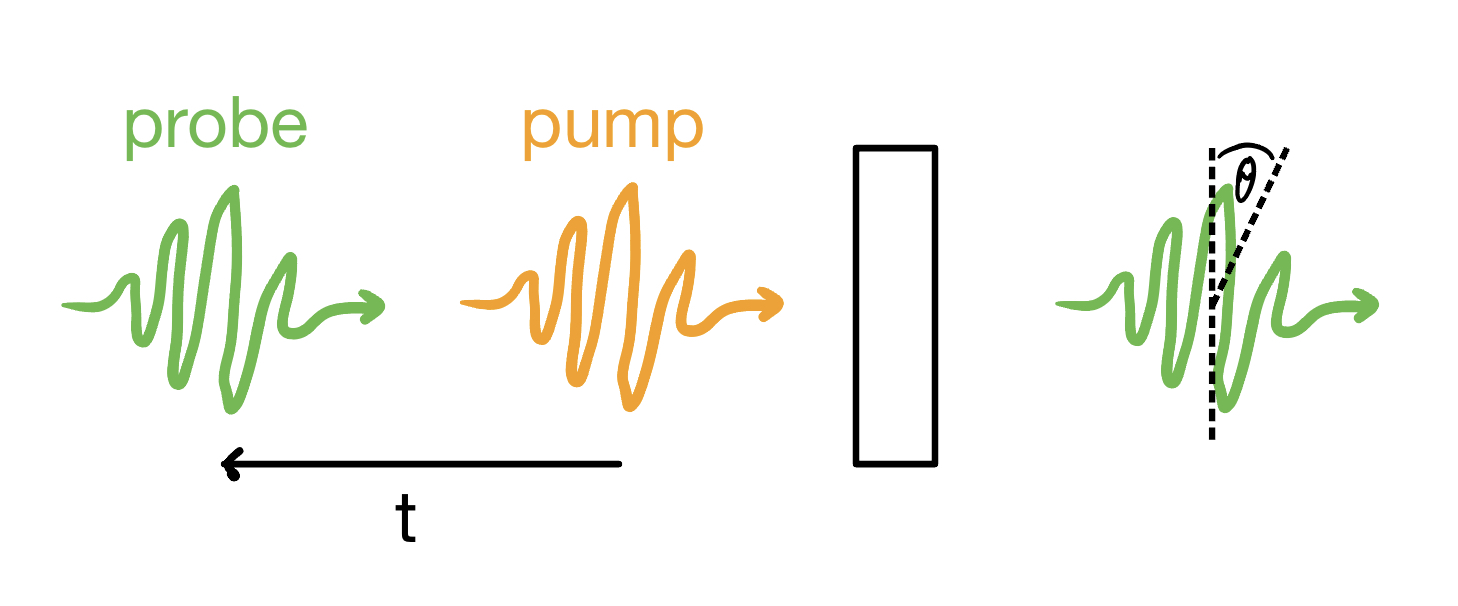
\includegraphics[width=0.6\textwidth]{pictures/pump_probe.jpeg}
    \caption{Schematic depiction of transmission pump-probe measurement.}
    \label{fig:pump_probe}
\end{figure}

\subsubsection*{Laser system}
Here a commercial ytterbium-based pulsed femtosecond laser (PHAROS) made by Light Conversion with a central wavelength of \qty{1028}{nm}, a pulse duration of about \qty{300}{fs} and a power of \qty{20}{W} is used.
With a repetition rate of \qty{50}{kHz} each pulse carries an energy of \qty{100}{\uJ}.
The Pharos output is split into two beams with \qty{7}{W} and \qty{13}{W}, of which the first one is designated to be the probe and the second to be the pump beam.
To ensure a separate tunability in wavelength of the two beams each one is fed into an optical parametric amplifier (OPA) Orpheus.
The OPA consists of a series of non-linear optics mounted on motorized stages, containing among others white light generation (WLG) and difference frequency generation (DFG).
The former of which makes it possible to select a specific signal frequency to amplify via the DFG process.
\begin{figure}[ht]
    \centering
    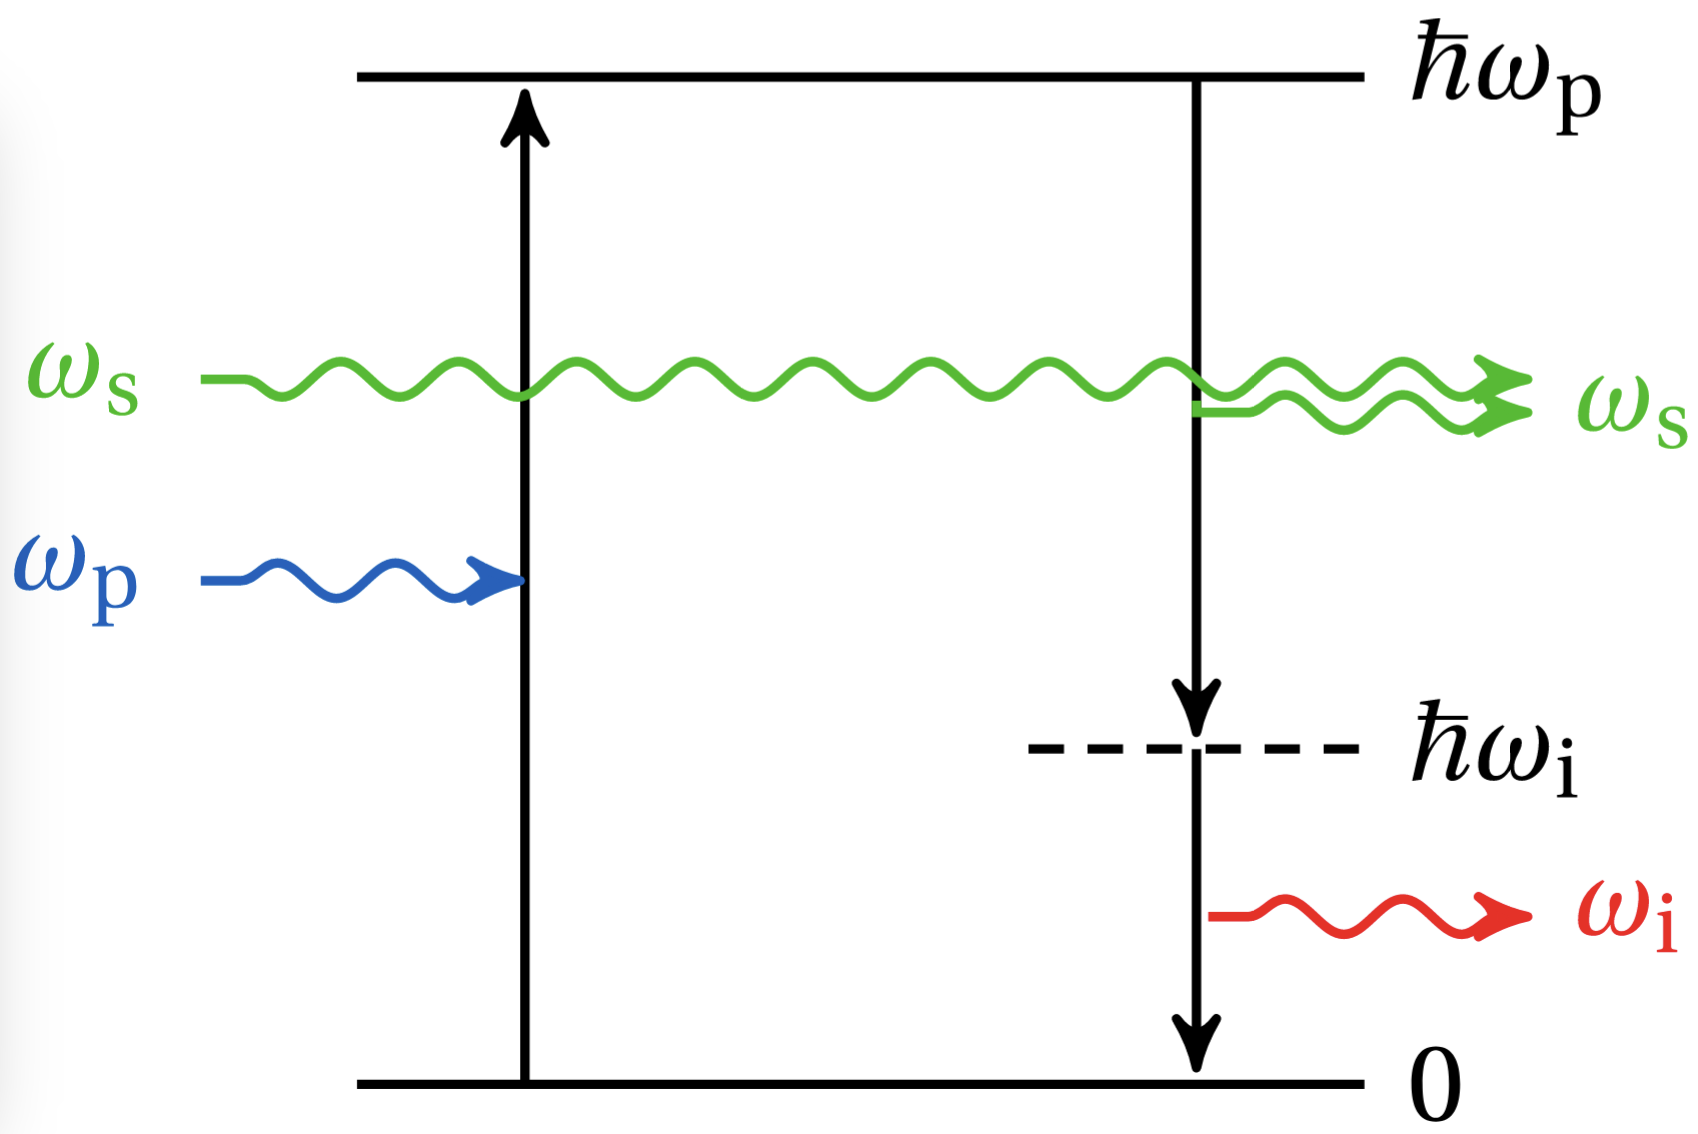
\includegraphics[width=0.5\textwidth]{pictures/OPA.png}
    \caption{Illustration of energetic transisions involved in the process of optical parametric amplification.}
    \label{fig:OPA}
\end{figure}
As can be seen in \autoref{fig:OPA} a pump beam is necessary to amplify the signal beam.
Another beam called idler is created as a byproduct, so that the following relation holds:
\begin{equation*}
    \omega_{\text{p}} = \omega_{\text{s}} + \omega_{\text{i}}
\end{equation*}
Before the OPA for the pump an electro optical modulator is placed only letting every second pulse pass.
This has the effect that half of the probe pulses encounter an unpumped sample, which sets a baseline for the detected signal.
The OPA also incorporates an internal compressor for the idler beam.
To compensate for the signal beam, its path can be manually adjusted via a quick replacement of mirrors to go through an external compressor.
Making up the last component of the stationary laser system is the external second harmonic generator (LYRA).
It extends the spectrum by twice reaching from \qty{0.5}{eV} to \qty{3.5}{eV}. 
\begin{figure}[ht]
    \centering
    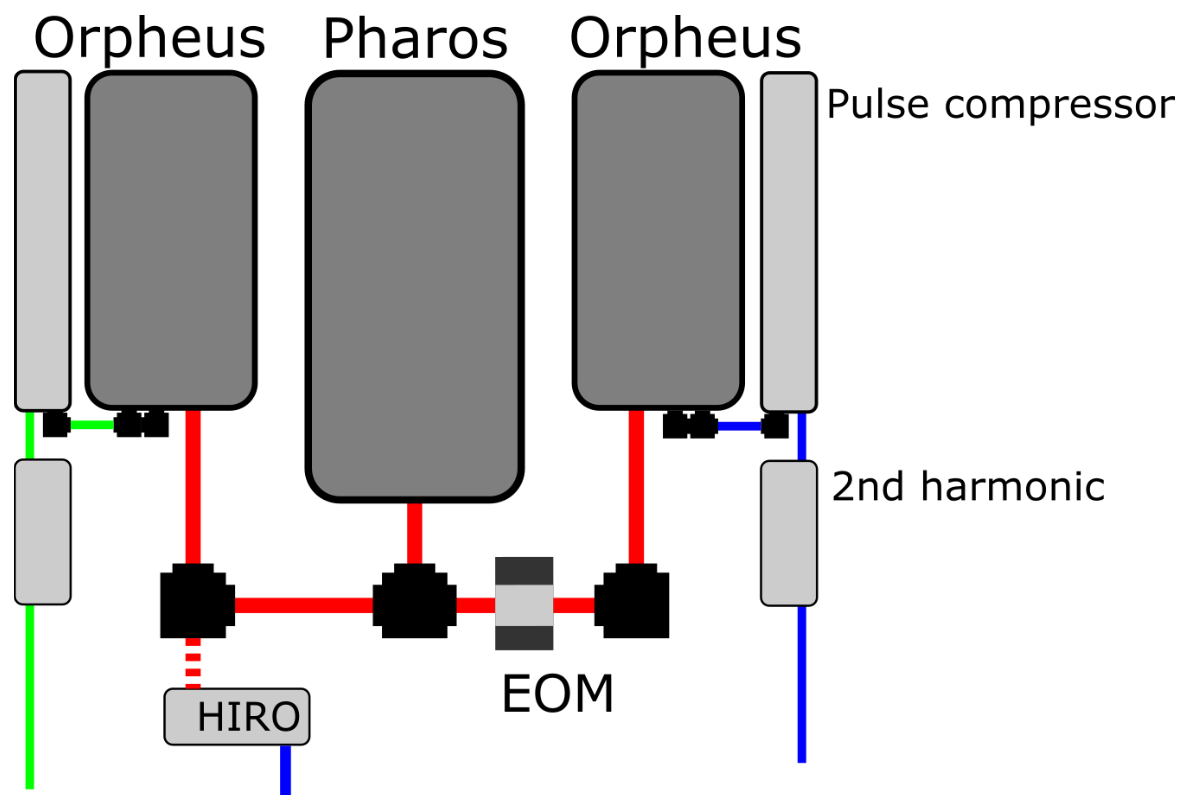
\includegraphics[width=0.65\textwidth]{pictures/laser_system.png}
    \caption{Schematic of the laser system containing labelled parts.}
    \label{fig:laser_systems}
\end{figure}
With the exception of the external compressor, the system can be operated with the corresponding desktop application and automatically adopts the typed-in wavelength.

\subsubsection*{Optical path}
As already mentioned above, a delayline is stationed in the pump beam path.
The pump travels the distance between the mirror and the delayline four times, which accounts for a factor of $\frac{4}{c}$ between the time delay and the shifted distance.
The laser light is horizontaly polarized to the plane of the table [PHAROS manual], so as an attenuator for the high peak power, a linear polarizer cube in combination with a $\frac{\lambda}{2}$-waveplate is used.
To vary the transmitting intensity the waveplate is rotated and to vary the angle of the light polarization for polarization dependent measurements an additional $\frac{\lambda}{2}$-waveplate is installed behind the attenuator.
Both the beams are then focused either by lenses or an objective on a common point on the sample surface, where a spatial overlap is achieved by using the computer-controlled piezo-driven mirror-holder from Newport.
% It is possible to use this system in the collinear, pump and probe are parallel, or the transversal, angle between pump and probe, scheme.
% The decision which geometry to incorporate is made based on the direction of the anisotropy.
Furthermore the setup can be adjusted for reflective or transmissive measurements.
The transmissive measurements being the more straightforward ones to implement wheras the reflective ones require the use of a beamsplitter to guide the light to the detection branch.

The sample is mounted in a open-loop cryostat requiring a steady flow of helium to reach and hold a desired temperature, which is essential for measurements exploring phase diagrams.
A magnetic valve controls the cross section of the supply pipe and thus the quantity of helium being pumped through the cryostat.
To maintain a specific steady temperature a heater governed by a PID controller is in thermal contact with the sample holder.
The cryostat itself is inserted inside a closed-loop, helium-cooled, superconductive magnet generating up to $\pm\qty{9}{T}$ at the sample position normal to the sample plane.
This allows for magnetic field dependence measurements, as well as for recording of hysteresis curves.
The sample stage has three axis and can be computer-controlled down to a stepsize of \qty{1}{nm} to shift to an exact position.

\subsubsection*{Data aquisition system}
MO effects typically induce a rotation of the polarization or ellipticity in the incident light and as most of the observed samples in the context of spintronics are rather thin, the change in the probe light often amounts to only a few mrad.
To overcome this issue, a specialised technique called balanced photodetection is used suppressing the background noise while simultaneously amplifying the difference between two incoming optical signals.
Firstly, the reflected or transmitted probe beam is guided through a $\frac{\lambda}{2}$-waveplate and a Wollaston prism.
The prism splits the light $I$ in two linearly polarized rays $I = I_p + I_s$ with their polarizations perpendicular to each other as depicted in \autoref{fig:balanced_detection}.
\begin{naligned}
    E_s &= E \cos\left(\sfrac{\pi}{4} + \theta\right) \\
    E_p &= E \sin\left(\sfrac{\pi}{4} + \theta\right)
    \label{eqn:balance}
\end{naligned}%
The waveplate is used to tilt the polarization of the light to such a degree that both of the rays hit the photodetector with the same intensity.
From this equilibrium position with a now switched on, previously arriving pump pulse, the polarisation of the probe gets rotated by an angle $\theta$.
This changes the ratio between the two photocurrents, which get converted into voltage and whose difference then gets amplified via operational amplifiers.
\begin{figure}[ht]
    \centering
    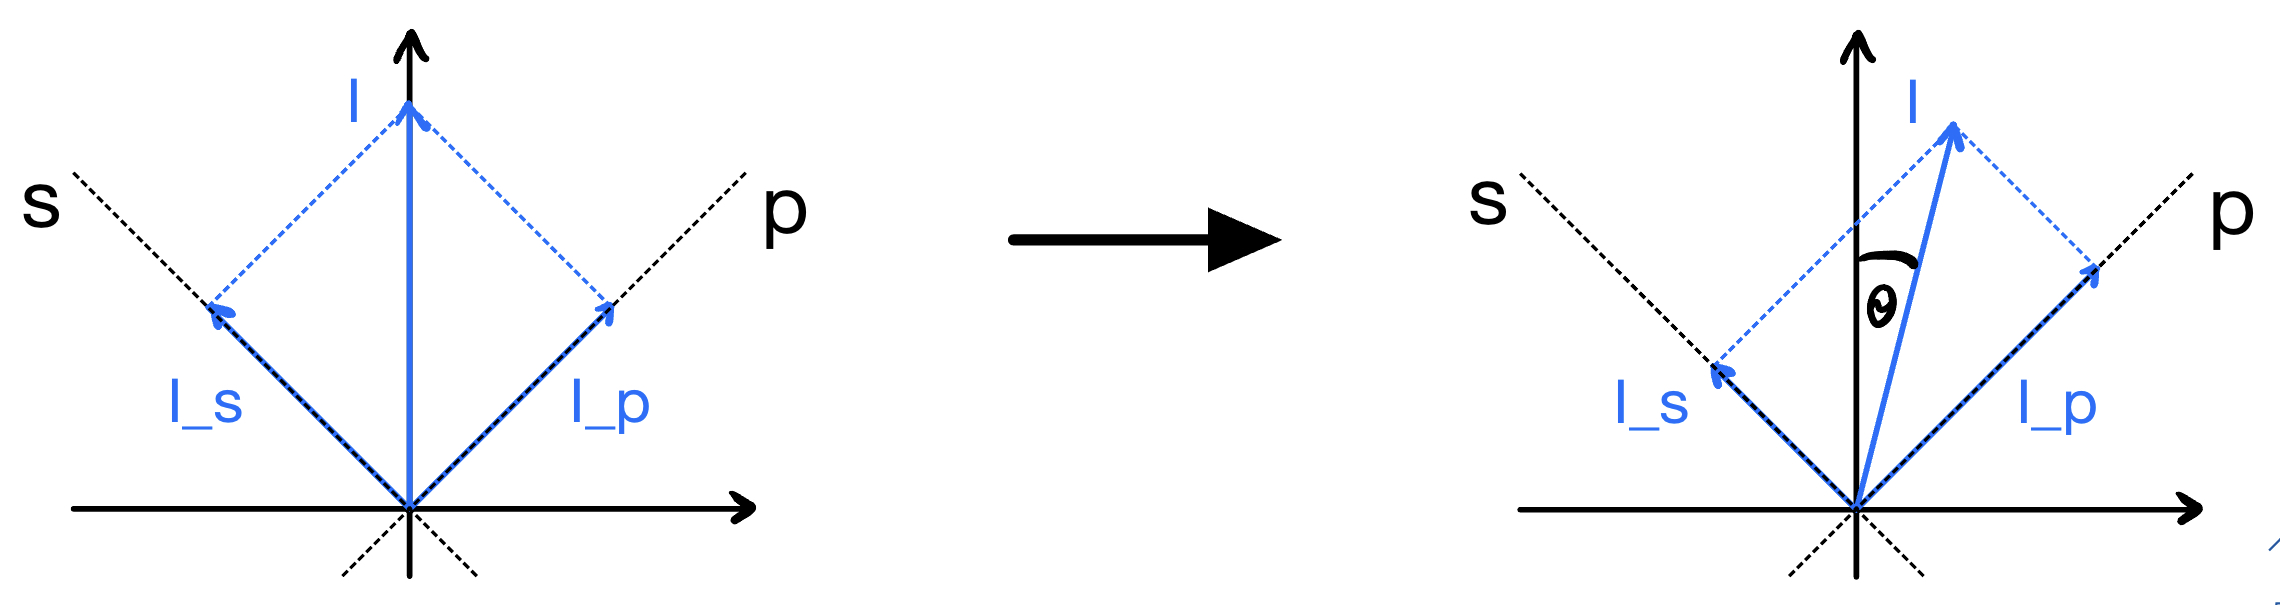
\includegraphics[width=\textwidth]{pictures/balanced_detection.jpeg}
    \caption{Representation how the incoming light gets split by the prism into two equally intense linearly polarized rays and how the subsequent rotation of polarisation materializes in the difference between s- and p-polarized light intensity.}
    \label{fig:balanced_detection}
\end{figure}
As the light is measured with a photodetector the incident light power is proportional to the generated current which in turn is proportional to the converted voltage and thus the signal observed on the computer.
Using this and \autoref{eqn:balance} the proportional  relation
\begin{equation}
    S \propto E_s^2 - E_p^2 \approx 2 E^2 \theta
\end{equation}
between a small angle $\theta$ and the signal $S$ can be derived.
% \chapter{Wichtige Hinweise zum Dokument}\label{make}

Diese Vorlage ist auf die Kompilierung mit \texttt{lualatex} ausgelegt. 
Als Dokumentenklasse  wird die \KOMAScript\-Klasse \texttt{scrbook} verwendet.
Falls Sie Änderungen am Layout vornehmen möchten, lesen Sie die \KOMAScript-Dokumentation: \cite{koma}.

Eine umfangreiche Einführung in die moderne Verwendung von \LaTeX{} gibt es hier: \cite{toolbox}, lesenswert ist außerdem das \LaTeX-Tabu: \cite{l2tabu}

Um dieses Dokument vollständig zu erstellen sind maximal vier Programmläufe nötig:
\begin{enumerate}[nosep]
    \item \texttt{lualatex BachelorArbeit.tex}
    \item \texttt{biber BachelorArbeit.bcf}
    \item \texttt{lualatex BachelorArbeit.tex}
    \item \texttt{lualatex BachelorArbeit.tex}
\end{enumerate}

Beim ersten Lauf des \LaTeX-Compilers werden die Kapitel, Links und zitierten Bibliographieeinträge in Hilfsdateien geschrieben.

Dann ist ein Lauf des Programms \texttt{biber} nötig, welches die benötigten Einträge aus der Hilfsdatei einliest, die Einträge aus der \texttt{.bib} Datei einliest, sortiert und formatiert und in eine weitere Hilfsdatei schreibt.

Beim nächsten \LaTeX-Lauf werden dann diese Hilfsdateien eingelesen und Literatur- und Inhaltsverzeichnis erstellt.

Manchmal ist ein vierter Lauf nötig, falls sich durch das einfügen des Literaturverzeichnisses Seitenzahlen verändert haben.

Das Tool \texttt{latexmk} übernimmt dies mit nur einem Programmaufruf und
führ nur so viele Aufrufe durch, wie nötig sind.

\texttt{latexmk --lualatex BachelorArbeit.tex}

Eine gute Option ist es, den \LaTeX{} Output in einem anderen 
Ordner zu erzeugen, dies ist mit der \texttt{--output-directory} Option möglich:

\texttt{latexmk --output-directory=build --lualatex BachelorArbeit.tex}


\section{Erstellen des Ausgabedokuments mit Make}

Für diese Vorlage wird ein Makefile zur Verfügung gestellt, welches automatisch alle Schritte ausführt, die für das fertige Dokument nötig sind.
Die Ausgabe erfolgt dabei in den Unterordner \texttt{build/}.
Make prüft, ob die Quelldateien verändert wurden, falls nicht, werden auch keine Befehle ausgeführt.

Falls Sie das Makefile benutzen möchten, sollten Sie alle Abhängigkeiten eintragen (Eigene Dateien für Kapitel, Plots, etc.).


Download und weitere Informationen zu Make gibt es unter \cite{make}. Die Befehle sind für die Bash ausgelegt.
Wenn Sie sie unter Windows nutzen wollen, benötigen Sie einen Bash-Emulator, wie Git Bash, Download unter \cite{gitbash} möglich.
Wenn Sie Make installiert haben, rufen Sie einfach in der Konsole im Verzeichnis der Arbeit den Befehl \texttt{make}.

\section{Erstellen des Ausgabedokuments mit Texmaker}
\subsection{Einrichten der nötigen Befehle}
Ein beliebter Editor für alle Betriebssysteme ist Texmaker, Download unter \cite{texmaker}.
Damit Texmaker das Dokument korrekt kompiliert, fügen sie einen benutzerdefinierten Befehl hinzu:
\begin{enumerate}[nosep]
    \item Klicken sie oben in der Menüleiste auf \emph{Benutzer/in}
    \item Klick auf \emph{Eigene Befehle}
    \item Klich auf \emph{Eigene Befehle editieren}, dort können Sie bis zu 5 eigene Befehle definieren
    \item Geben Sie dem Befehl unter \emph{Menüeintrag} einen Namen und tragen sie folgende Befehle in das Befehlsfeld ein: \\
      \small\verb+latexmk --lualatex --interaction=batchmode --halt-on-error %.tex |+
    \item Bestätigen Sie mit \emph{OK}
\end{enumerate}

\begin{figure}
    \centering
    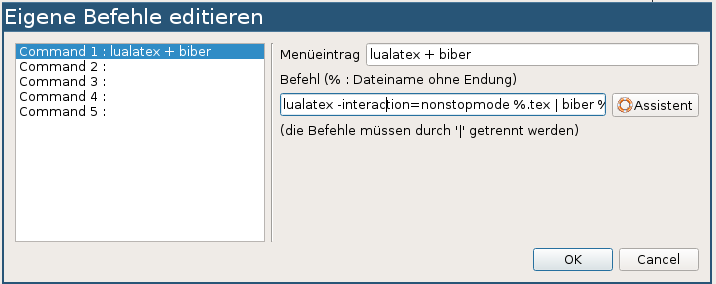
\includegraphics[width=12cm]{Plots/texmaker.png}
    \caption{Screenshot zur Erstellung des Kompilier-Befehls in Texmaker}
    \label{fig:texmaker}
\end{figure}


In Abbildung \ref{fig:texmaker} ist ein Screenshot des Befehlsmenü gezeigt. Ihren Befehl können Sie nun im Drop-Down-Menü zum 
Kompilieren des Dokuments auswählen und mit einem Klick auf den Pfeil starten.

\subsection{Aufräumen}

Nach einem \LaTeX-Fehler ist es oft notwendig, die erstellten Hilfsdateien zu löschen.
Klicken Sie hierzu auf \emph{Werkzeuge}→\emph{Aufräumen}.


\chapter{\LaTeX-Grundlagen}

Bitte beachten Sie beim Schreiben der Arbeit folgende Konventionen bzw. Grundlagen:

\begin{itemize}
    \item \textbf{Abschnitte und Zeilenumbrüche} \\
        Es sollten im Fließtext keine Zeilenumbrüche mit \textbackslash\textbackslash \ erzwungen werden.
        Schreiben Sie höchsten einen Satz in eine Code-Zeile.
        Absätze werden im Code mit einer Leerzeile markiert und dann entsprechend der Einstellung von \texttt{parskip} in der Dokumentenklasse gesetzt.
    \item \textbf{Kursiv/Aufrecht} \\
        \begin{itemize}
            \item Variablen und physikalische Größen werden kursiv gesetzt. 
            \item Einheiten werden immer aufrecht und mit einem halben Leerzeichen Abstand zur Zahl gesetzt. Nutzen Sie \texttt{siunitx}!
            \item Mathematische Konstanten und Funktionen werden ebenfalls aufrecht gesetzt. Zum Beispiel die Eulersche Zahl e, das imaginäre i und das infinitesimale d.
                Im Mathematikmodus können Sie dies mit dem Befehl \verb_\mathrm{}_ erreichen. Für die Funktionen stellt \LaTeX \ Befehle bereit, z.B. \verb+\arccos+.
            \item Integrand und ein $\mathrm{d}x$ sollten ebenfalls durch ein kleines Leerzeichen (\verb+\,+) getrennt werden.
        \end{itemize}
        


\end{itemize}

\section{Zahlen und Einheiten}

Jede Zahl, jede Einheit und jede Zahl mit Einheit sollte mit Hilfe der in dem Paket \texttt{siunitx} zur Verfügung gestellten Befehle gesetzt werden.
Grundsätzlich gilt: Einheiten werden aufrecht gesetzt und haben ein kleines Leerzeichen (\verb+\,+) Abstand zu ihrer Zahl. 
Werden Fließkommazahlen ohne \texttt{siunitx} gesetzt, entsteht ein hässlicher Leerraum zwischen Komma und erster Nachkommastelle, da \LaTeX \ das Komma nicht als Dezimaltrennzeichen, sondern als Satzzeichen interpretiert.

Das Paket wurde mit deutschen Spracheinstellungen (also mit Komma als Dezimaltrennzeichen und $\cdot$ zwischen Zahl und Zehnerpotenz) geladen, sowie mit den Einstellungen, dass die Standardabweichung stets durch $\pm$ abgetrennt wird und Einheiten falls nötig als Brüche ausgegeben werden.

\begin{table}
    \centering
    \caption{Beispiele für siunitx}
    \label{tab:si}
    \begin{tabular}{l r}
        \toprule
        Befehl     &   Ergebnis \\
        \midrule
        \verb+\num{1.2345}+ & \num{1.2345} \\
        \verb+\num{1.2e3}+ & \num{1.2e3} \\
        \verb_\num{1.2 +- 0.2}_ & \num{1.2+-0.2} \\
        \verb+\num{10000}+ & \num{10000} \\
        \verb+\si{\meter\per\second}+ & \si{\meter\per\second} \\
        \verb+\SI{1.2(1)}{\micro\ampere}+ & \SI{1.2(1)}{\micro\ampere} \\
        \verb+\SI{1.2\pm0.1e3}{\kilo\gram\per\cubic\meter}+ & \SI{1.2\pm0.1e3}{\kilo\gram\per\cubic\meter} \\
        \bottomrule 
    \end{tabular}
\end{table}

Das Paket stellt unter anderem die drei wichtigen Befehle
\begin{itemize}
    \item \texttt{\textbackslash num\{Zahl\}},
    \item \texttt{\textbackslash si\{Einheit\}} und
    \item \texttt{\textbackslash SI\{Zahl\}\{Einheit\}}
\end{itemize}
zur Verfügung.
Diese Befehle sollten stets genutzt werden, wenn Zahlen angegeben werden. 
Sie funktionieren sowohl im Text- als auch im Mathematikmodus.
In Tabelle \ref{tab:si} sind einige Beispiele aufgetragen. Bitte lesen Sie die Dokumentation \cite{siunitx}.

\section{Das Literaturverzeichnis}

Das Literaturverzeichnis wird mit Hilfe von BibLaTeX und biber erstellt.
Tragen Sie alle ihre Quellen in die Datei \texttt{references.bib} ein, Sie enthält bereits
einige Beispiele. Für weitere Informationen lesen Sie bitte die Dokumentation \cite{biblatex}.

Im Text können Sie mit \verb_\cite{kürzel}_ zitieren. Seitenzahlen geben Sie in eckigen Klammern an:
\verb_\cite[10]{kürzel}_. 

Das Literaturverzeichnis ist so eingestellt, dass es Ihre Quellen in alphabetischer Reihenfolge nach Autoren nummeriert.
Möchten Sie das Literaturverzeichnis nach der Reihenfolge des Auftauchens im Text sortieren, fügen sie die Paktetoption \texttt{sorting=none} beim Laden
des BibLaTeX-Pakets hinzu.

Den Zitier- und Bibliographie-Stil geben sie mit der Option \texttt{style=Stil} an. Die beiden gebräuchlisten Stile sind \texttt{numeric} und \texttt{alphabetic}. 
Bei \texttt{numeric} werden die Quellen durchnummeriert, bei \texttt{alphabetic} wird ein Buchstabenkürzel aus Autor(en)-Name(n) und Jahr verwendet.
Für weitere Stile konsultieren Sie bitte die Dokumentation: \cite{biblatex}.

Ein Beispiel für das Zitieren eines Buches lautet so \cite{handbook_adhesives},
wissenschaftliche Artikel hingegen werden so \cite{einstein} zitiert.

Damit das Literaturverzeichnis erstellt wird, ist ein Aufruf von \texttt{biber} nach einem ersten kompilieren mit \texttt{lualatex} nötig.
Danach muss das Dokument erneut mit \texttt{lualatex} kompiliert werden. 

Zum korrekten Kompilieren des Dokuments siehe Kapitel \ref{make}.

% \chapter{Abbildungen und Tabellen}

\section{Abbildungen}

Achten Sie bei ihren Plots auf ausreichend große Achsenbschriftungen, ausreichende Schriftdicken und gut unterscheidbare Farben.
Im Idealfall haben Sie im Plot und der Arbeit die gleiche Schriftgröße und Schriftart.
Dies lässt sich durch Erstellen des Plots in der korrekten Größe und Einbinden mit dem optionalen Argument \texttt{scale=1} erreichen. Ein Beispiel sehen Sie in Abbildung \ref{fig:bsp}.

Nutzen Sie wenn möglich Vektorgrafiken (pdf) und nur in Ausnahmen Rastergrafiken wie .png oder .jpg.
Setzen Sie Punkte hinter Abbildungsunterschriften.

\begin{figure}
    \centering
    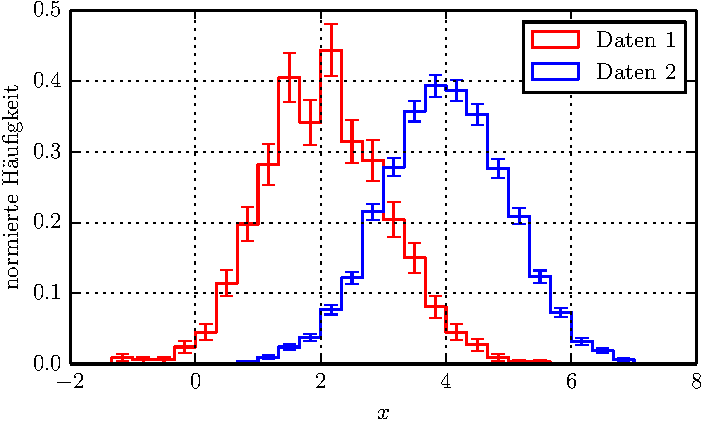
\includegraphics[scale=1]{./Plots/Histogramm.pdf}
    \caption{Ein Histogramm mit Fehlerbalken für zwei Datensätze, Schriftgröße und -art entsprechen der des Dokuments.}
    \label{fig:bsp}
\end{figure}

\section{Tabellen}

Tabellen sollten so einfach wie möglich aufgebaut sein, verzichten Sie auf zu viele Linien. In fast allen Fällen reichen drei horizontale Linien aus, jeweils über und unter der Tabelle und zwischen den Spaltenüberschriften und der eigentlichen Tabelle.

Das Paket \texttt{booktabs} stellt hierfür \verb_\toprule_, \verb_\midrule_ und 
\verb_\bottomrule_ zur Verfügung.
Das Paket \texttt{siunitx} stellt eine extrem mächtige neue Spalteneinstellung bereit: \texttt{S}, mit ihr können Zahlen und Einheiten sehr sauber und gut ausgerichtet gesetzt werden.

Diese Vorlage geht von Tabellenüberschriften aus, möchten Sie dagegen Tabellenunterschriften entfernen Sie das entsprechende optionale Argument für die Dokumentenklasse in der Präambel.

Ein Beispiel ist Tabelle~\ref{tab:bsp}.
\begin{table}
    \centering
    \caption{Beispieltabelle mit willkürlichen Werten, für die Zahlenwerte wurde die S-Option aus \texttt{siunitx} verwendet.}
    \label{tab:bsp}
    \begin{tabular}{S[table-format=4.2] S[table-format=3.2]}
        \toprule
        {$p \mathrel{/} \si{\pascal}$}  & {$T \mathrel{/} \si{\kelvin}$} \\
        \midrule
        1024,23 & 273,15 \\
        1025,31 & 274,5 \\
        1026,27 & 276,2 \\
        \bottomrule
    \end{tabular}
\end{table}


% \appendix
% Hier beginnt der Anhang, nummeriert in lateinischen Buchstaben
% \chapter{Ein Anhangskapitel}

Hier könnte ein Anhang stehen, falls Sie z.\,B.\ Code, Konstruktionszeichnungen oder Ähnliches mit in die Arbeit bringen wollen.
Im Normalfall stehen jedoch alle Ihre Resultate im Hauptteil der Bachelorarbeit und ein Anhang ist überflüssig.


\backmatter
\printbibliography

% \cleardoublepage
% From https://www.tu-dortmund.de/studierende/im-studium/pruefungsangelegenheiten/allgemeine-vordrucke/
% 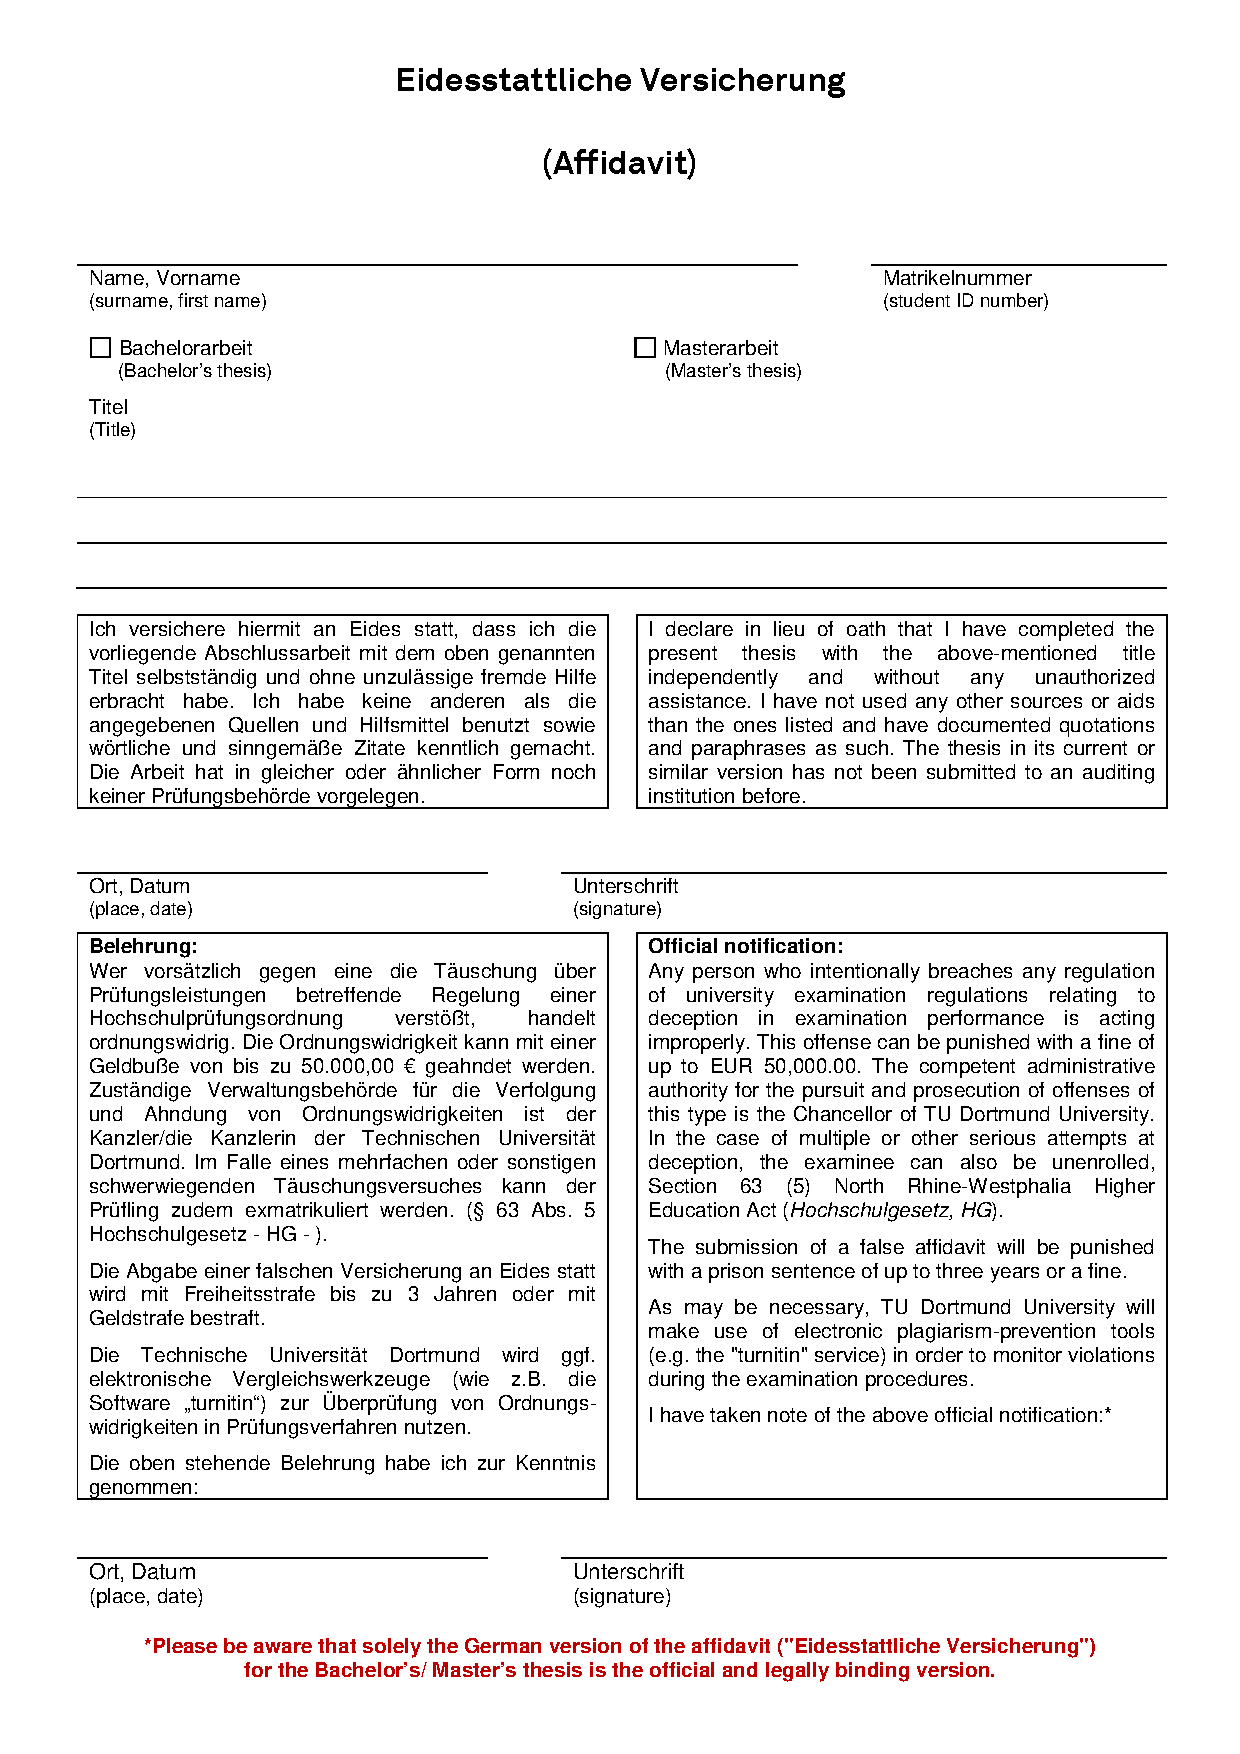
\includepdf{content/Eidesstattliche_Versicherung.pdf}

\end{document}
